\subsection{Acceptance correction}
\label{sec:kpimm:acceptance}

The triggering, reconstruction and selection of candidates distort the distributions of the decay angles \ctl, \ctk, $\phi$, as well as the \qsq and \mkpi distributions, leading to acceptance effects. The dominant sources of bias derive from the track momentum and impact parameter requirements. 

In order to take into account acceptance effects, a five dimensional efficiency function is determined from simulated four-body \BdToKpimm decays generated according to a phase space distribution. If the distributions of \qsq, \ctl, \ctk, $\phi$ and \mkpi were all generated flat, the distributions of the variables after reconstruction and selection would give the shape of the efficiency.  While this is true for \ctl, \ctk and $\phi$, it is not the case for \qsq and \mkpi. Therefore, the simulated candidates are reweighted in order to transform the reconstructed distributions to the efficiency shape.

The efficiency is parameterised in terms of orthonormal Legendre polynomials of order $n$, $L_n(x)$, as
\begin{equation}
\begin{split}
\varepsilon(\qsq',\ctl,&\ctk,\phi',\mkpi') = \\
& \sum_{hijkl} c_{hijkl}~L_{h}(\qsq')L_{i}(\ctl)L_{j}(\ctk)L_{k}(\phi')L_{l}(\mkpi').
 \end{split}
 \label{eqn:legendre}
\end{equation}
As the polynomials are orthonormal over the domain $x\in[-1,1]$, the variables $\qsq'$, $\phi'$ and $\mkpi'$ are used, which are obtained by linearly transforming \qsq, $\phi$ and \mkpi to lie in this range.

The coefficients $c_{hijkl}$ are determined using a moment analysis of simulated four-body \BdToKpimm phase-space decays as

\begin{equation}
   \begin{split}
     c_{h,i,j,k,l} = \frac{1}{\sum w_{n}}\sum_{n=0}^{N}&w_{n}\left(\frac{2h+1}{2}\right)\left(\frac{2i+1}{2}\right)\left(\frac{2j+1}{2}\right)\left(\frac{2k+1}{2}\right)\left(\frac{2l+1}{2}\right)\\
     &\times L_{h}(\qsq)L_{i}(\ctl)L_{j}(\ctk)L_{k}(\phi)L_{l}(\mkpi)~,
     \end{split}
 \end{equation}

\noindent where $w_{n}$ is the per-candidate weight taking into account both the non-flat distributions of \qsq and \mkpi, and the candidate weights described in Sec.~\ref{sec:kpimm:data-mc:reweight}. The factors of $(2a + 1)/2$ arise from the orthogonality of the Legendre polynomials,
 
\begin{equation}
\int_{-1}^{+1} L_{a}(x) L_{a'}(x) \deriv x = \frac{2}{2 a + 1}\delta_{ a a'}  ~.
\end{equation}

 The sum in Eq.~\ref{eqn:legendre} encompasses $L_n(x)$ up to fourth order in \ctl and $\mkpi'$, sixth order in $\phi'$ and $\qsq'$, and eighth order in \ctk. The order of polynomial used in each case is the lowest order possible that gives good agreement between the efficiency function and the simulated four-body \BdToKpimm phase-space decays. The angular acceptance in the decay angles \ctl, \ctk and $\phi'$ in the region $1.1<\qsq<6.0\gevgevcccc$, $1330<\mkpi<1530\mevcc$ is shown in Fig.~\ref{fig:acceptance}.

\begin{figure}[!htb]
  \centering
  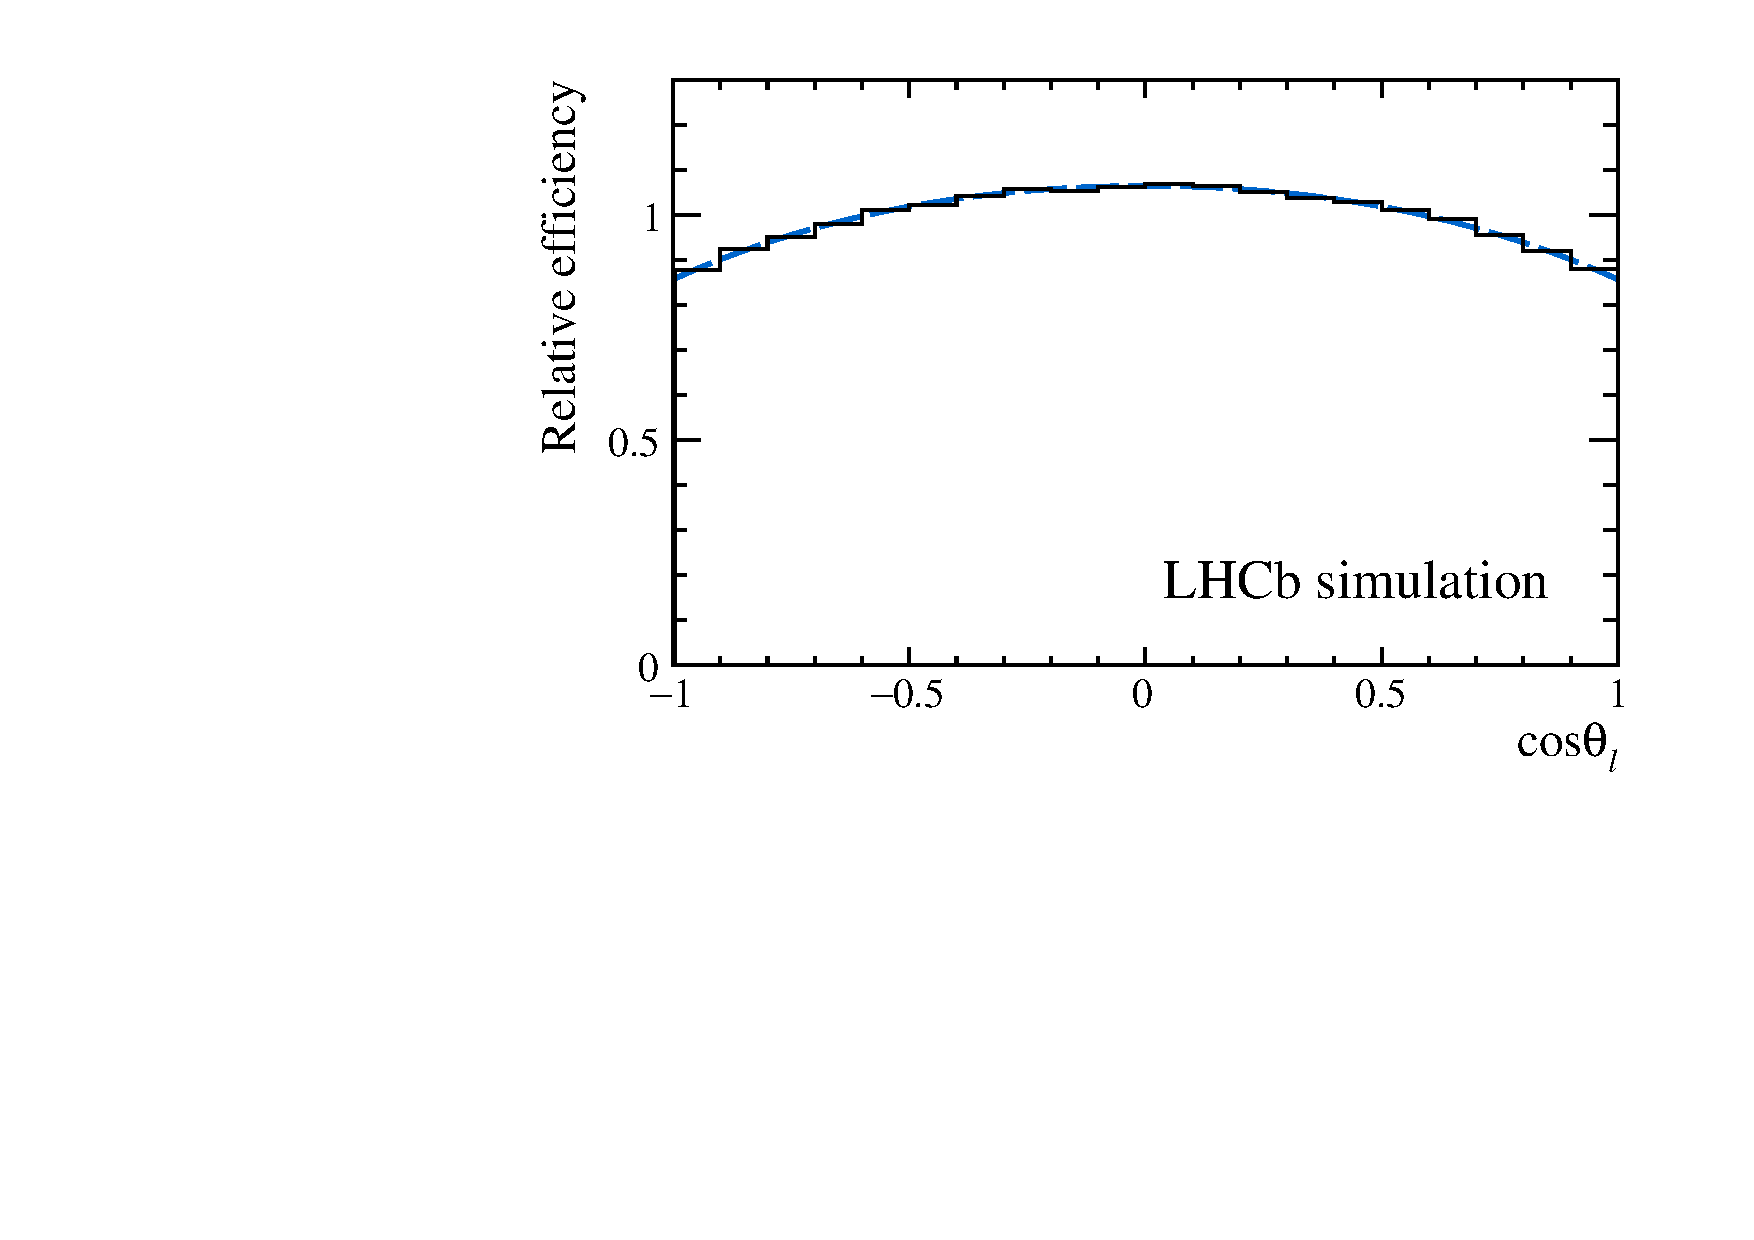
\includegraphics[width=0.49\linewidth]{figs/kpimm/acceptance/ctl.pdf}
  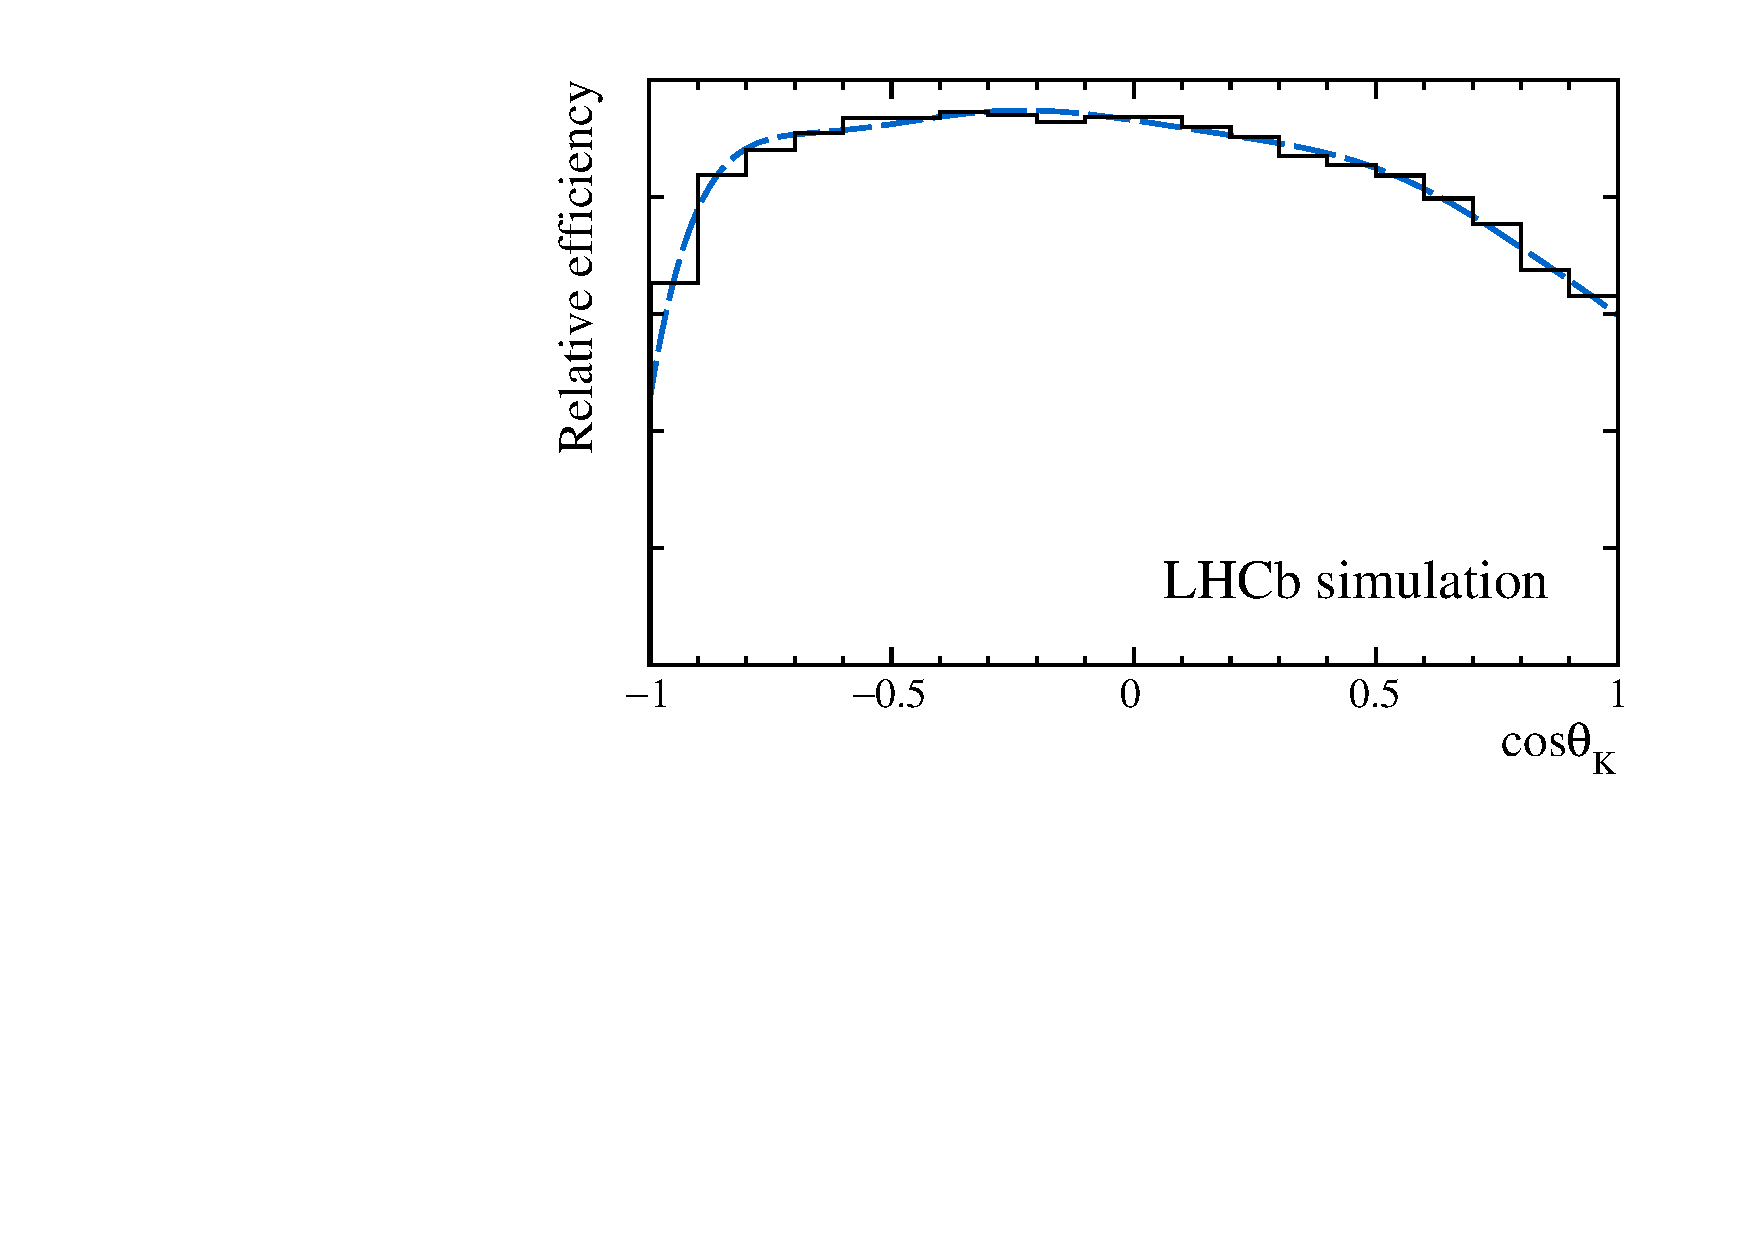
\includegraphics[width=0.49\linewidth]{figs/kpimm/acceptance/ctk.pdf}\\
  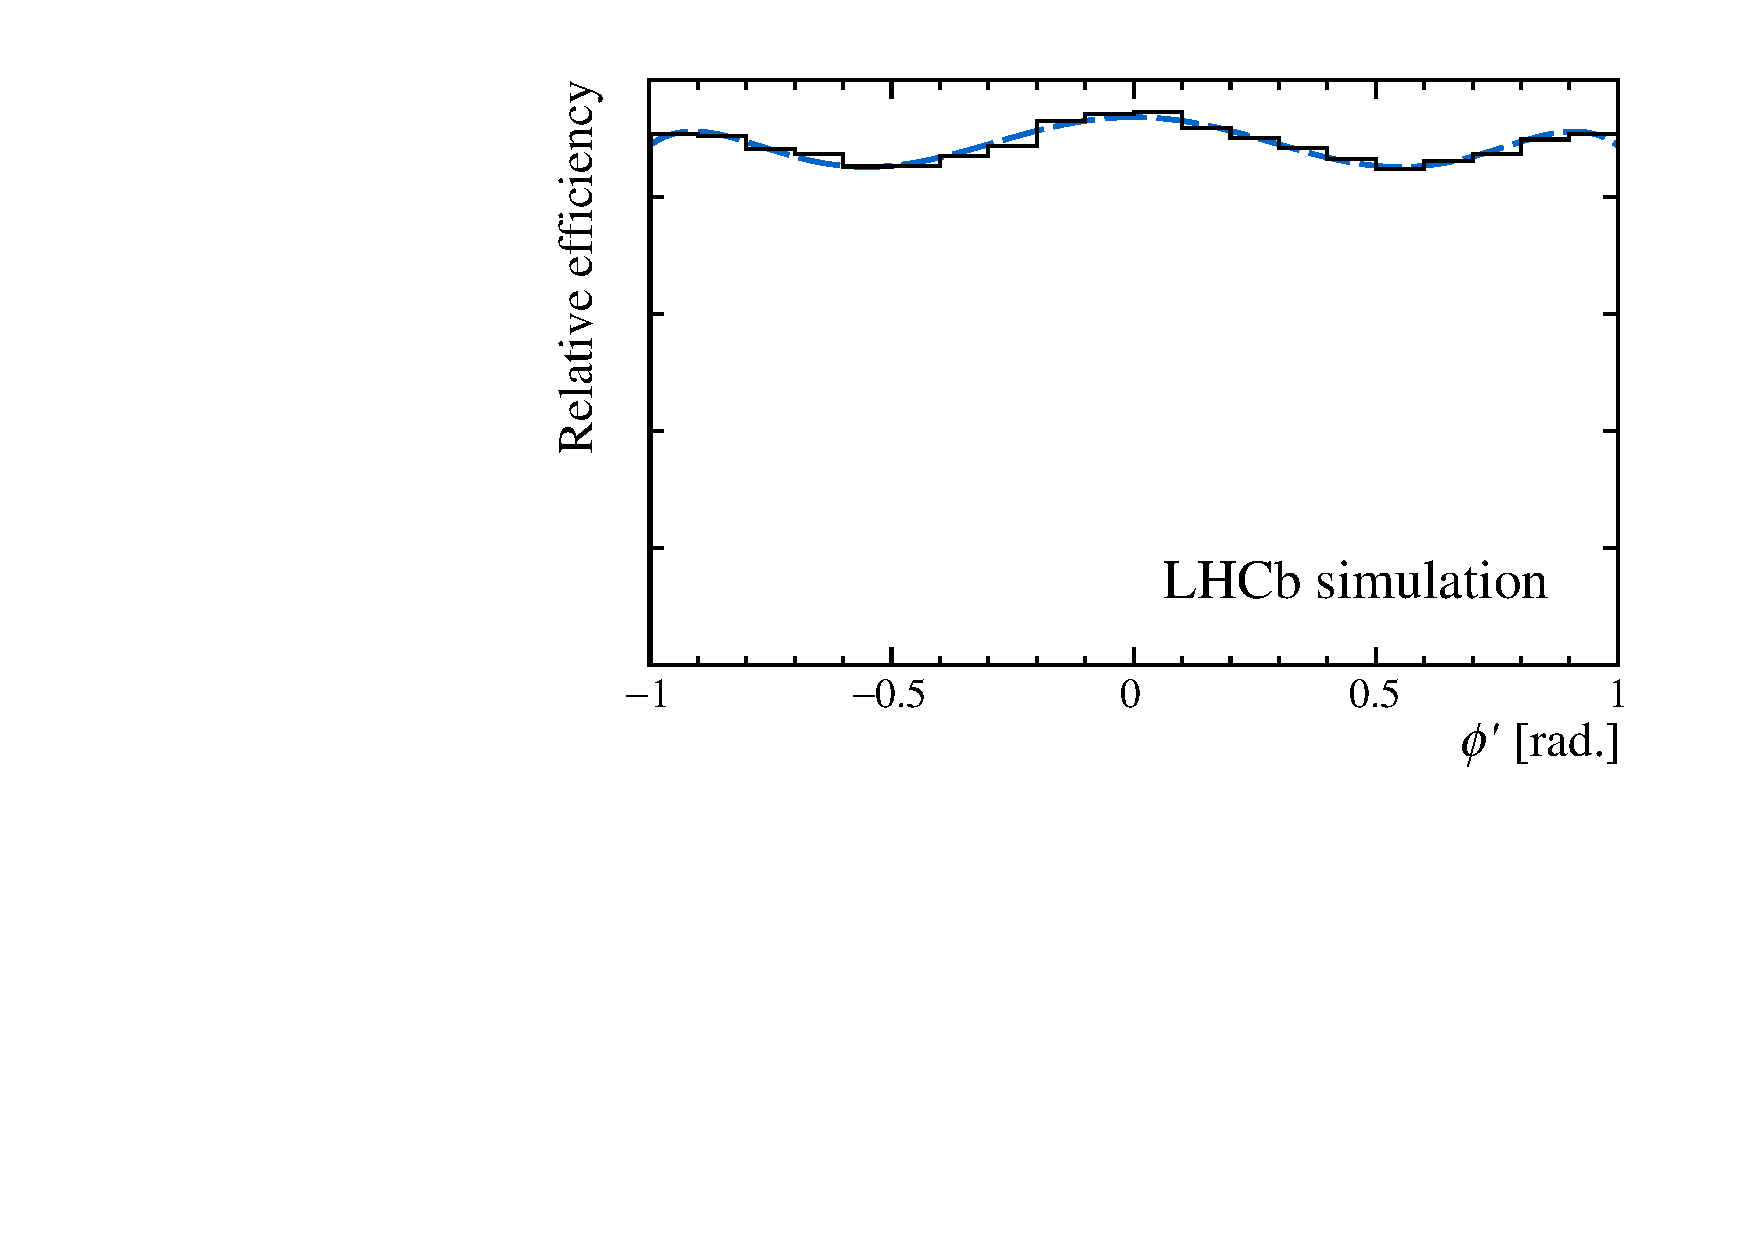
\includegraphics[width=0.5\linewidth]{figs/kpimm/acceptance/phi.pdf}
  \caption{Relative efficiency in \ctl, \ctk and $\phi'$ in the region $1.1<\qsq<6.0\gevgevcccc$ and $1330<\mkpi<1530\mevcc$ as determined from a moment analysis of simulated four-body \BdToKpimm decays. The efficiency function is shown by the dashed blue line.  The solid histograms indicate the distribution of simulated four-body \BdToKpimm phase-space decays used to determine the acceptance.}
\label{fig:acceptance}
\end{figure}